\documentclass{beamer}

\usepackage{amsmath}
\usepackage{xcolor}
\usepackage{graphicx}
\usepackage{cite}
\usepackage{amsmath}
\usepackage{pgfplots}
\usepackage[absolute,overlay]{textpos}



\usepackage{ragged2e}
\justifying

\usetheme[progressbar=frametitle]{metropolis}
\setbeamertemplate{frame numbering}[fraction]
\useoutertheme{metropolis}
\useinnertheme{metropolis}
\usefonttheme{metropolis}
\usecolortheme{spruce}
\setbeamercolor{background canvas}{bg=white}

%\usetheme{Warsaw}
%\usecolortheme{crane}
\definecolor{mygray}{rgb}{0.3,0.3,0.3}
\usecolortheme[named=mygray]{structure}


\title[Reinforcement Learning]{A Self-organized Sensor Data Path Selection Method in Internet of Things}
\author{Milad Khademi Nori}
\institute{Amirkabir University of Technology}
\date{\today}
\begin{document}

\begin{frame}
\titlepage
\end{frame}


\begin{frame}[t]{Agenda} %\vspace{10pt}
\begin{itemize}
\item Energy Harvesting Wireless Sensor Networks (EH-WSNs)
		\begin{itemize}
		\item Applications of EH-WSNs 
		\item Components of EH-WSNs
		\item Problems of EH-WSNs
		\end{itemize}		
\item Current protocols for EH-WSNs
		\begin{itemize}		
		\item Classical protocols
		\item Non-classical protocols
		\item Pros and cons of current protocols
		\end{itemize}		
\item Our proposed protocol
		\begin{itemize}
		\item The main superiority of our protocol
		\end{itemize}
\item Conclusion
\end{itemize}
\end{frame}


\begin{frame}[t]{Energy Harvesting Wireless Sensor Networks (EH-WSNs)} %\vspace{10pt}
\textbf{Applications of EH-WSNs}
\begin{itemize}
\item Smart parking
	\begin{itemize}
	\justifying
	\item It is necessary to deploy a number of nodes which can check the presence of cars in different locations [1].
	\end{itemize}
\item Smart agriculture
	\begin{itemize}
	\justifying
	\item To measure a couple of parameters in different parts of the farmland such as the humidity of the soil, the temperature, and the intensity of sunlight [1].
	\end{itemize}
\item And so on ...
\end{itemize}
\end{frame}


\begin{frame}[t]{Energy Harvesting Wireless Sensor Networks (EH-WSNs)} %\vspace{10pt}
\textbf{Components of EH-WSNs}: 
\small
they consist of a large number of nodes. These nodes are equipped with following 5 units [2]:\\
$\bullet$ A central processing unit \hspace{25pt} $\bullet$ A wireless transceiver unit \\
$\bullet$ One or multiple sensors unit \hspace{11pt} $\bullet$ An energy storage unit \\
$\bullet$ An energy harvesting unit \textbf{(the source of energy!)}
\begin{center}
\includegraphics[scale=0.3]{figure/NodeFig}
\end{center}
\end{frame}



\begin{frame}[t]{Energy Harvesting Wireless Sensor Networks (EH-WSNs)} %\vspace{10pt}
\textbf{Problems of EH-WSNs}
\small
\begin{itemize}
\justifying
\item Even though EH-WSNs could harvest energy from the environment, the collected energy and the real demand do not meet because of stochastic nature of harvested energy, thus such networks suffer from intermittent failure [2].
\item Due to the limited range of EH-WSNs, they rely on multihop transmission to deliver their packets to the base station located far away [2].
\item \textbf{Therefore protocols should support multihop transmission and perform as energy-efficient as possible.}
\item Protocols are either \textbf{flat} or \textbf{hierarchical} [1].
\item It has been shown that hierarchical protocols are significantly more energy-efficient than flat protocols [1].
\end{itemize}
\end{frame}


\begin{frame}[t]{Current protocols for EH-WSNs} %\vspace{10pt} 
\small
\begin{itemize}
\justifying
\item In hierarchical protocols, two decisions mainly determine the energy-efficiency of the protocols [1].
	\begin{itemize}
	\item Clustering: it divides the network into some separate clusters.
	\item Cluster Head Selection: it defines the CH of each cluster
	\end{itemize}
\end{itemize}

\begin{center}
\includegraphics[scale=0.19]{figure/FlatHier}
\end{center}

\begin{center}
\includegraphics[scale=0.45]{figure/Phase}
\end{center}

\end{frame}


\begin{frame}[t]{Current protocols for EH-WSNs} %\vspace{10pt}
\small
\quad $\bullet$ Non-classic protocols (LEACH [3], DEARER [1], EPSO-CEO [4], and WOA-C [5])\\
\quad \quad $\bullet$ Pros	\\
\quad \quad \quad	$\bullet$ {\color{green} They do not rely on GPS.}	\\
\quad \quad $\bullet$ Cons \\
\quad \quad \quad $\bullet$ {\color{red} They form inefficient clusters.} \\
\quad $\bullet$ Classic protocols (KCA [6] and Mk-means [7])\\
\quad \quad $\bullet$ Pros	\\
\quad \quad \quad	$\bullet$ {\color{green} They can form clusters efficiently.}	\\
\quad \quad $\bullet$ Cons \\
\quad \quad \quad $\bullet$ {\color{red} They rely on GPS module [8].} \\
\quad \quad \quad \quad $\bullet$ {\color{red} GPS increases implementation cost [8].}\\
\quad \quad \quad \quad $\bullet$ {\color{red} GPS increases energy consumption [8].}\\
\quad \quad \quad \quad $\bullet$ {\color{red} GPS works poorly in indoor applications [8].}\\
\end{frame}

\begin{frame}[t]{Our proposed protocol} %\vspace{10pt}
\small
\begin{itemize}
\justifying
\item {\color{green} Our proposed protocol clusters the whole network efficiently using agglomerative clustering without assuming that nodes are equipped by GPS.}
\item {\color{green} It selects reliable CHs which lead to the lowest energy consumption according to an ILP optimization problem using QGSA.} 
\item It consists of eight steps which seven of them are just done at the initialization phase, the last step is required to be operated at the beginning of each round.
\item Our game changer is the mathematical idea that a noisy or semi-complete Euclidean distance matrix could be reconstructed by an acceptable accuracy.
\end{itemize}
\end{frame}

\begin{frame}[t]{Our proposed protocol} %\vspace{10pt}
\begin{center}
\includegraphics[scale=0.51]{figure/Steps.pdf}
\end{center}
\end{frame}

\begin{frame}[t]{Our proposed protocol} %\vspace{10pt}
\begin{center}
\includegraphics[scale=0.51]{figure/Output.pdf}
\end{center}
\end{frame}


\begin{frame}[t]{Our proposed protocol} %\vspace{10pt}
\textbf{Steps of our protocols}
\begin{enumerate}
\justifying
\small
\item RSSI vector measurement and collection.
\begin{equation}
        \left\{ \begin{array}{ll}
    		\hat{s}_{1}=[\cdot]_{(N+1)\times1}     & \textrm{node number $1$}\\
    		\vdots                                  & \quad \vdots \\
    		\hat{s}_{(N+1)}=[\cdot]_{(N+1)\times1}   & \textrm{node number $(N+1)$}
        \end{array} \right.
\end{equation}
\item Transmission of RSSI vector collection to the BS.
\item Distance estimation based on RSSI [9].
\begin{equation}
        \left\{ \begin{array}{ll}
    		\hat{d}_{1}=[\cdot]_{(N+1)\times1}     & \textrm{node number $1$}\\
    	    \vdots                            &\quad \vdots \\
    		\hat{d}_{(N+1)}=[\cdot]_{(N+1)\times1}   & \textrm{node number $(N+1)$}
        \end{array} \right.
\end{equation}
\item The BS merges all vectors into an incomplete EDM.
\begin{equation}
\hat{D}=[\hat{d}_{1},\hat{d}_{2},\cdots,\hat{d}_{(N+1)}]_{(N+1)\times(N+1)}
\end{equation}
\end{enumerate}		
\end{frame}


\begin{frame}[t]{Our proposed protocol} %\vspace{10pt}
\begin{itemize}
\justifying
\small
\item The BS completes the incomplete EDM by solving EDM completion problem [10].
\begin{equation}
\hat{D} \Longrightarrow  D
\end{equation}
\item The BS applies agglomerative clustering and forms clusters.
\begin{equation}
J_{opt}=\sqrt{\frac{N \varepsilon_{fs}}{2\pi \varepsilon_{mp}}}\frac{L}{d_{toBS}^{2}}
\end{equation}
\item The BS forms a tree using the minimum cost spanning tree to enable intercluster communication.
\begin{equation}
m_{ij}=\frac{1}{C_i C_j}\sum_{k=1}^{C_i}\sum_{l=1}^{C_j}D_{kl}
\end{equation}
\item The BS selects the optimal CH for each cluster.
\begin{equation}
minimize\quad R(\ell)\sum_{i=1}^{C_{j}}x_i(\Lambda_{ij}+\Delta_{ij}(\ell))
\end{equation}
\end{itemize}

\end{frame}

\begin{frame}[t]{Our proposed protocol} %\vspace{10pt}
\begin{itemize}
\small
\justifying
\item $\Lambda_{ij}$ is the energy consumption of members of the $j$th cluster in case the $i$th node in the cluster is selected as the CH which is calculated as follows:
\begin{equation}
\Lambda_{ij}(\ell)=\sum_{k\neq i}^{C_j} \Gamma_{ki}(d_{ki})
\end{equation}
\item And $\Delta_{ij}(\ell)$ is the energy consumption of the CH is given by:
\begin{equation}
\Delta_{jn}= \Psi_{jn}+ \Omega_{jn}
\end{equation}
\item where $\Psi_{jn}$ is the energy to receive data from its members aggregate and forward them to the next hop ($n$), $\Omega_{jn}$ is the energy to receive packets of its subclusters and relay them to the next hop. $\Psi_{jn}$ is calculated as follows:
\begin{equation}
\Psi_{jn}=L_p(C_j-1)e_{elec}+L_pC_je_{da}+\Gamma_{jn}(d_{jn})
\end{equation}
\end{itemize}
\end{frame}


\begin{frame}[t]{Our proposed protocol} %\vspace{10pt}
\begin{itemize}
\small
\justifying
\item where $L_p(C_j-1)e_{elec}$ is the energy consumption to receive packets from $(C_j-1)$ members, $L_pC_je_{da}$ is the amount of energy required to perform data aggregation, and $L_p\Gamma_{jn}(d_{jn})$ is the required energy to send them to the next hop. $\Omega_{jn}$ is calculated as follows:
\begin{equation}
\Omega_{jn}=Z_jL_pe_{elec}+Z_j\Gamma_{jn}(d_{jn})
\end{equation}
\item where $Z_jL_pe_{elec}$ is the energy consumption to receive packets from $Z_j$ subclusters, $Z_j\Gamma_{jn}(d_{jn})$ is the energy required to send them to the next hop. Consequently, the energy update function for the $j$th CH node is given by:
\begin{equation}
E_j(\ell+1)=E_j(\ell)+H_j(\ell)-R(\ell)\times \Delta_{jn}
\end{equation}
\end{itemize}
\end{frame}


\begin{frame}[t]{Our proposed protocol} %\vspace{10pt}
\begin{itemize}
\small
\justifying
\item Reliability constraint is that the sum of RE and harvested energy minus energy consumption ($\Delta_{ij}(\ell)$) for the CH during $\ell$th round should be positive which is as follows:
\begin{equation}
subject\ to\quad \sum_{i=1}^{C_j}x_i\Big(E_i(\ell)+H_i(\ell)-R(\ell)\Delta_{ij}(\ell)\Big)\geq0
\label{eq:const1}
\end{equation}
\begin{equation}
\sum_{i=1}^{C_j}x_i=1, \quad x_i\in \{0,1\}
\label{eq:const2}
\end{equation}
\item Equation \ref{eq:const1} implies that for the selected CH in the $j$th cluster sum of RE and harvested energy should be more than energy consumption to guarantee reliability. Equation \ref{eq:const2} limits the ILP to select one node as CH.
\end{itemize}
\end{frame}

\begin{frame}[t]{Our proposed protocol} %\vspace{10pt}
\begin{itemize}
\small
\justifying
\item But as large ILPs are generally intractable, using approximation methods or heuristic methods (e.g., simulated annealing, particle swarm, ant colony, etc) instead of deterministic methods could decrease the com- putational effort and processing time.
\item We employ a QGSA approach which is a binary method. On the other hand, our problem is a binary problem so utilizing QGSA for our problem is appropriate.
\item Although metaheuristic algorithms do not guarantee the optimality, they give a sub-optimal solution in a reasonable amount of time.

\end{itemize}
\end{frame}


\begin{frame}[t]{Our proposed protocol} %\vspace{10pt}
\textbf{Numerical Experiment}
\begin{itemize}
\small
\justifying
\item The network energy efficiency $\eta$ is the ratio between the number of successfully delivered packets throughout the network lifetime and the total harvested energy by all nodes during the network lifetime. The \emph{Energy Efficiency} is defined as follows [1]:
\begin{equation}
\eta=\lim_{L\to\infty}\frac{\sum_{\ell=1}^{L}\sum_{i=1}^{N}P_{i}(\ell)}{\sum_{\ell=1}^{L}\sum_{i=1}^{N}H_{i}(\ell)} \quad (Packet/Joule)
\end{equation}
\item The packet loss percentage $\zeta$ is the ratio between failed packets throughout the network lifetime and total generated packets by nodes. The \emph{Packet Loss Percentage} is defined as follows [1]:
\begin{equation}
\zeta=\lim_{L\to\infty}\frac{\sum_{\ell=1}^{L}\sum_{i=1}^{N}P_{i}(\ell)}{\sum_{\ell=1}^{L}\sum_{i=1}^{N}A_{i}(\ell)} 
\end{equation}
\end{itemize}
\end{frame}

\begin{frame}[t]{Our proposed protocol} %\vspace{10pt}
\begin{figure}
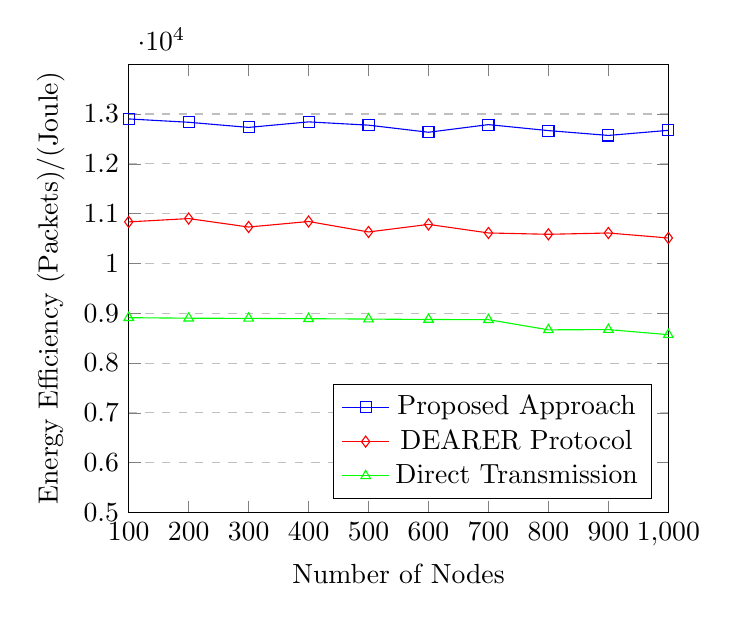
\begin{tikzpicture}
\begin{axis}[
    %title={Energy Efficiency},
    xlabel={Number of Nodes},
    ylabel={Energy Efficiency (Packets)/(Joule)},
    xmin=100, xmax=1000,
    ymin=5000, ymax=14000,
    xtick={100,200,300,400,500,600,700,800,900,1000},
    ytick={3000,4000,5000,6000,7000,8000,9000,10000,11000,12000,13000},
    legend pos=south east,
    ymajorgrids=true,
    grid style=dashed,
]
 
\addplot[
    color=blue,
    mark=square,
    ]
    coordinates {
    (100,12901)(200,12834)(300,12731)(400,12842)(500,12776)(600,12634)(700,12787)(800,12667)(900,12570)(1000,12672)
    };
    \addlegendentry{Proposed Approach}
    
\addplot[
    color=red,
    mark=diamond,
    ]
    coordinates {
    (100,10834)(200,10901)(300,10731)(400,10842)(500,10632)(600,10784)(700,10612)(800,10585)(900,10611)(1000,10511)
    };
    \addlegendentry{DEARER Protocol}    
    
\addplot[
    color=green,
    mark=triangle,
    ]
    coordinates {
    (100,8911)(200,8901)(300,8897)(400,8891)(500,8883)(600,8875)(700,8871)(800,8667)(900,8672)(1000,8570)
    };
    \addlegendentry{Direct Transmission }     
    
\end{axis}
\end{tikzpicture}
\end{figure}
\end{frame}

\begin{frame}[t]{Our proposed protocol} %\vspace{10pt}
\begin{figure}[!t]
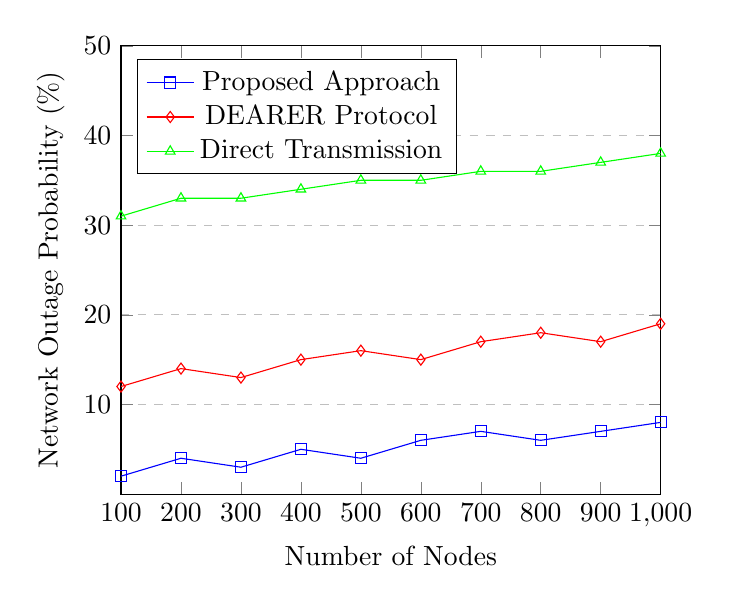
\begin{tikzpicture}
\begin{axis}[
    %title={Outage Probability},
    xlabel={Number of Nodes},
    ylabel={Network Outage Probability (\%)},
    xmin=100, xmax=1000,
    ymin=0, ymax=50,
    xtick={100,200,300,400,500,600,700,800,900,1000},
    ytick={10,20,30,40,50,60,70,80,90,100},
    legend pos=north west,
    ymajorgrids=true,
    grid style=dashed,
]
 
\addplot[
    color=blue,
    mark=square,
    ]
    coordinates {
    (100,2)(200,4)(300,3)(400,5)(500,4)(600,6)(700,7)(800,6)(900,7)(1000,8)
    };
    \addlegendentry{Proposed Approach}
    
\addplot[
    color=red,
    mark=diamond,
    ]
    coordinates {
    (100,12)(200,14)(300,13)(400,15)(500,16)(600,15)(700,17)(800,18)(900,17)(1000,19)
    };
    \addlegendentry{DEARER Protocol}    
    
\addplot[
    color=green,
    mark=triangle,
    ]
    coordinates {
    (100,31)(200,33)(300,33)(400,34)(500,35)(600,35)(700,36)(800,36)(900,37)(1000,38)
    };
    \addlegendentry{Direct Transmission }     
    
\end{axis}
\end{tikzpicture}
\end{figure}
\end{frame}

\begin{frame}[t]{Conclusion} %\vspace{30pt}
\begin{itemize}
\small
\justifying
\item We have proposed a protocol which even though does not rely on GPS can benefit from a classical clustering approach.
\item Our game changer is the mathematical idea that a noisy or semi-complete Euclidean distance matrix could be reconstructed by an acceptable accuracy.
\item We have formulated the CH selection problem as an ILP problem and solved it by QGSA.
\item The results show that the proposed approach surpasses current approaches which do not assume that nodes are equipped GPS.
\end{itemize}
\end{frame}

\begin{frame}[t]{Conclusion} \vspace{30pt}
\Huge
\begin{center}
Any Question?
\end{center}
\end{frame}

\begin{frame}[t]{References}
\tiny
[1] Y. Dong, J. Wang, B. Shim, and D. I. Kim, “Dearer: A distance-and-energy-aware routing with energy reservation for energy harvesting wireless sensor networks,” IEEE Journal on Selected Areas in Communications, vol. 34, no. 12, pp. 3798–3813, Dec 2016.

[2] D. Wu, J. He, H. Wang, C. Wang, and R. Wang, “A hierarchical packet forwarding mechanism for energy harvesting wireless sensor networks,” IEEE Communications Magazine, vol. 53, no. 8, pp. 92–98, August 2015.

[3] W. R. Heinzelman, A. Chandrakasan, H. Balakrishnan, Energy-efficient communication protocol for wireless microsensor networks, in: System sciences, 2000. Proceedings of the 33rd annual Hawaii international conference on, IEEE, 2000, pp. 10–pp.

[4] J. RejinaParvin and C. Vasanthanayaki, “Particle swarm optimization-based clustering by preventing residual nodes in wireless sensor networks,” IEEE Sensors Journal, vol. 15, no. 8, pp. 4264–4274, Aug 2015.

[5] A. R. Jadhav and T. Shankar, “Whale optimization based energy-efficient cluster head selection algorithm for wireless sensor networks,” CoRR, vol. abs/1711.09389, 2017. [Online]. Available: http://arxiv.org/abs/1711.09389

[6] J. Wang, K. Wang, J. Niu, W. Liu, A k-medoids based clustering algorithm for wireless sensor networks, in: 2018 International Workshop on Advanced Image Technology (IWAIT), 2018, pp. 1–4.

[7] S. Periyasamy, S. Khara, S. Thangavelu, Balanced cluster head selection based on modified k-means in a distributed wireless sensor network 2016 (2016) 1–11.

[8] S. K. Singh, P. Kumar, J. P. Singh, A survey on successors of leach protocol, IEEE Access 5 (2017) 4298–4328.

[9] Y. Miao, H. Wu, L. Zhang, The accurate location estimation of sensor node using received signal strength measurements in large-scale farmland, Journal of Sensors 2018.

[10] A. Tasissa and R. Lai, “Exact reconstruction of euclidean distance geometry problem using low-rank matrix completion,” CoRR, vol. abs/1804.04310, 2018.

\end{frame}

\end{document}